%% author_tex.tex
%% V1.0
%% 2013/04/06
%%
%% This file describes the coding for oupau.cls

\documentclass[times]{oupau}

\usepackage{natbib}
\graphicspath{ {figs/} }

%The author can find the documentation of the above style file and any additional
%supporting files if required from "http://www.ctan.org"

% *** Do not adjust lengths that control margins, column widths, etc. ***

\begin{document}
\renewcommand{\thefigure}{S\arabic{figure}}

\runningheads{C. M. Guimond \textit{et al.}}{Rocky planet oxygen fugacities supplement}

\title{{\LARGE Supplement to}\\{\Large How oxidising are exoplanet mantles? Variability constraints and compositional trends}}

\author{Claire Marie Guimond\affil{a,}\footnote{Correspondence to: cmg76@cam.ac.uk},
Oliver Shorttle\affil{a,b}, Sean Jordan\affil{b}, and  John F. Rudge\affil{a}}

\address{\affilnum{a}\emph{Department of Earth Sciences, University of Cambridge, Downing Street, Cambridge CB2 3EQ, UK}\\
\affilnum{b}\emph{Institute of Astronomy, University of Cambridge, Madingley Road, Cambridge CB3 0HA, UK}}
% \corraddr{Corresponding author address. E-mail: cmg76@cam.ac.uk}

% \begin{abstract}
% Insert your abstract text. Insert your abstract text. Insert your abstract text. Insert your abstract text.
% Insert your abstract text. Insert your abstract text. Insert your abstract text. Insert your abstract text.
% Insert your abstract text. Insert your abstract text. Insert your abstract text. Insert your abstract text.
% Insert your abstract text. Insert your abstract text. Insert your abstract text. Insert your abstract text.
% \end{abstract}

% \keywords{Insert keywords here}

% \received{Insert article history}
%\revised{<As needed>}
%\accepted{<As needed>}

\maketitle

\section{Supplementary Figures}

\begin{figure}[!h]
         \centering
         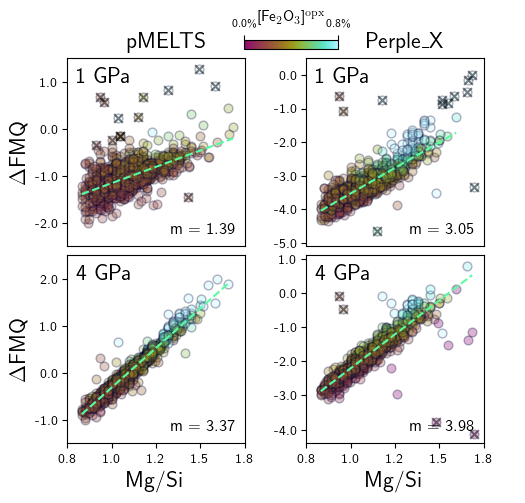
\includegraphics[width=0.6\textwidth]{figs/crossplot_mgsi_fit.png}
        \caption{The same cross-plots as the left columns of Figures 3 and 4 in the main text but with linear regressions overlain in green: mantle oxygen fugacity, expressed as $\Delta$FMQ, as a function of the mantle molar Mg/Si ratio. Outliers (grey crosses), as determined by their effects on $\chi^2$ using a leave-one-out method, are excluded from the regressions.        Slopes $m$ of the regressions are shown in the bottom right corner of each panel. Calculations are performed at $1373\,\text{K}$ and at $1\,{\rm GPa}$ \textit{(top)} and $4\,{\rm GPa}$ \textit{(bottom)}, using pMELTS \textit{(left)} and the \citet{jennings_simple_2015} database in Perple\_X \textit{(right)}. Each point represents a bulk mantle composition estimated from refractory element abundances of planet-hosting stars in the Hypatia Catalog \citep{hinkel_stellar_2014}.}
        \label{fig:mgsi_fit}
\end{figure}

\begin{figure}[!h]
         \centering
         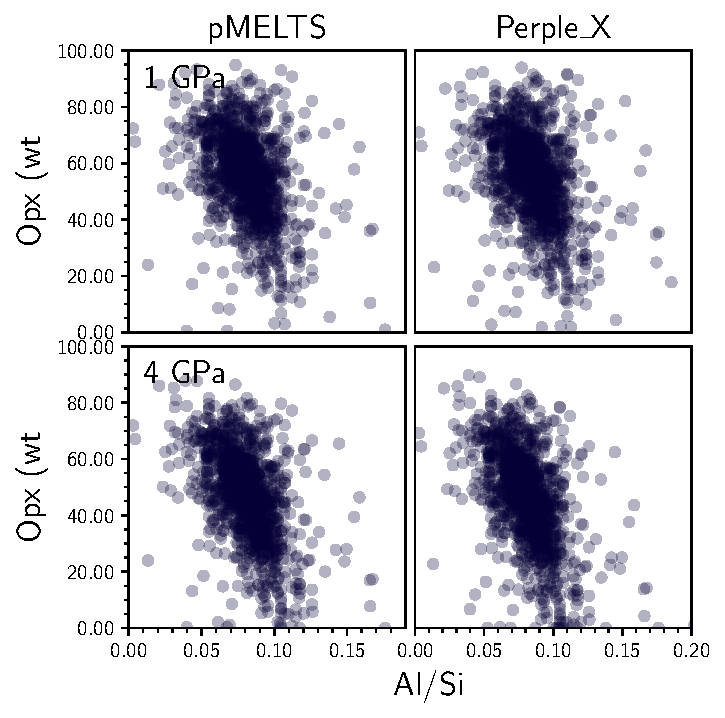
\includegraphics[width=0.6\textwidth]{figs/crossplot_al_opx.pdf}
        \caption{Cross-plot of the wt.\% modality ratios of an aluminous phase (spinel, Sp, or garnet, Gt) to orthopyroxene (Opx), as a function of the molar Al/Si ratio, estimated for rocky exoplanet mantles and based on refractory element abundances from planet-hosting stars in the Hypatia Catalog \citep{hinkel_stellar_2014}, here assuming an Earth-like molar ratio of core Fe-metal to mantle FeO. Calculations are performed at $1373\,\text{K}$ and at $1\,{\rm GPa}$, nominally the spinel field \textit{(top)}, or $4\,{\rm GPa}$, nominally the garnet field \textit{(bottom)}, using pMELTS \textit{(left)} and the \citet{jennings_simple_2015} database in Perple\_X \textit{(right)}. Note a few extreme cases are not visible in these $y$-axis limits. With increasing Al/Si, higher proportions of the aluminous phase are stabilised at the expense of orthopyroxene.}
        \label{fig:alsi_opx}
\end{figure}
\clearpage

\bibliographystyle{mnras}
\bibliography{references.bib}

\end{document}